\documentclass[aspectratio=169,11pt]{beamer}
\usetheme{default}
\setbeamertemplate{navigation symbols}{}
\setbeamertemplate{footline}[frame number]
\setbeamercolor{frametitle}{fg=black!85}

\usepackage{graphicx}
\usepackage{booktabs}
\usepackage{amsmath}
\graphicspath{{figures/}}

\title{Outer pressure boundary, and pulses at hot walls}
\subtitle{Follow-up on your boundary formulas}
\author{Keheng Zhu}
\date{27 October 2026}

\begin{document}

\begin{frame}
  \titlepage
\end{frame}

%----------------------------------------------------------------------
\begin{frame}{Two questions, short answers}
  \begin{enumerate}
    \item \textbf{Fix only $T$ at the top?} (so AWSoM-R need not give $p$)\\[0.2em]
          $\to$ One condition goes missing. Evaporation drops $\approx12\times$;
          mass drains out of the bottom.
    \vspace{0.8em}
    \item \textbf{Velocity pulses at hot walls (100\,kK): physical?}\\[0.2em]
          $\to$ Numerical: halving the cells doubles their frequency.
  \end{enumerate}
\end{frame}

%----------------------------------------------------------------------
\begin{frame}{The model}
  \begin{itemize}
    \item 1-D column, 1600\,km (mid-chromosphere) to 2153\,km (\textbf{domain top},
          22\,kK initially).
    \item Single fluid, Saha hydrogen, gravity, conduction
          $\kappa = \kappa_e + \kappa_n$ (electrons + neutral H). No radiation.
    \item Top ghost cells: \textbf{wall temperature} $T_{\rm wall}$ (22--100\,kK).
          It heats the column and drives evaporation.
    \item Mesh: 276\,m cells near the top (``N500'').
  \end{itemize}
\end{frame}

%======================================================================
\begin{frame}
  \centering\Large Part 1: the outer boundary
\end{frame}

%----------------------------------------------------------------------
\begin{frame}{Today: $p$ and $T$ both fixed at the top}
  \centering
  \begin{tabular}{@{}l l l@{}}
    \toprule
    ghost cells & top (outflow) & bottom (inflow) \\
    \midrule
    pressure    & fixed, 0.0103\,Pa & fixed \\
    temperature & fixed, $T_{\rm wall}$ & fixed, 6.6\,kK \\
    velocity    & copied from top cell & 0 \\
    \bottomrule
  \end{tabular}
  \vspace{1.2em}

  Subsonic outflow: one incoming characteristic. Over-specified?
\end{frame}

%----------------------------------------------------------------------
\begin{frame}{Your formulas}
  $b$ = ghost cell, $n$ = last cell, $\Delta x$ between centres, $p=\rho RT$.
  \vspace{-0.4em}
  \begin{align*}
    \text{equation of state:}\quad & p_b = \rho_b R_b T_b \\
    \text{hydrostatic balance:}\quad & p_n - p_b = \tfrac12(\rho_n+\rho_b)\,g\,\Delta x \\[0.3em]
    \text{substitute } p_b:\quad & p_n - \rho_b R_b T_b = \tfrac12\rho_n g\Delta x + \tfrac12\rho_b g\Delta x \\
    \text{collect } \rho_b:\quad & \rho_b\left(R_bT_b + \tfrac12 g\Delta x\right) = p_n - \tfrac12\rho_n g\Delta x \\
    \Rightarrow\quad & \boxed{\rho_b = \frac{p_n - \tfrac12\rho_n g\,\Delta x}{R_bT_b + \tfrac12 g\,\Delta x}}
  \end{align*}
  \vspace{-0.3em}
  Only $T_b$ is imposed; $\rho_b$ follows from the last cell, then $p_b = \rho_b R_b T_b$.
\end{frame}

%----------------------------------------------------------------------
\begin{frame}{Counting (1): pure Euler}
  \[
    w_\pm = \delta p \pm \rho c\,\delta u,\qquad w_s = \delta p - c^2\delta\rho
  \]
  \[
    \frac{\delta T}{T} = \frac{\gamma-1}{\gamma}\,\frac{w_+ + w_-}{2p} + \frac{w_s}{\gamma p}
  \]
  \begin{itemize}
    \item Only $w_-$ enters. $\delta T=0$ fixes it $\Rightarrow$
          \alert{$T$ alone is a valid condition for Euler.}
    \item But for an isothermal wave ($\gamma\to1$), $T$ cannot see it.
  \end{itemize}
\end{frame}

%----------------------------------------------------------------------
\begin{frame}{Counting (2): with conduction}\label{fr:count2}
  \begin{itemize}
    \item Energy equation becomes 2nd order in $T$ $\Rightarrow$ +1 condition per end.
    \item Remaining waves travel at $u\pm c_T$ (isothermal) $\Rightarrow$ 1 more enters.
    \item[$\Rightarrow$] Outflow needs \alert{2 independent conditions}.
          $T$ fills one; the other must be $p$, $\rho$ or $w_-$.
  \end{itemize}
  \vspace{0.6em}
  {\small (Count after Strikwerda 1977; the $c_T$ step is mine. Please check.)}
\end{frame}

%----------------------------------------------------------------------
\begin{frame}{Why $T$ cannot count twice}
  \begin{itemize}
    \item $T_b = T_{\rm wall}$ is \textbf{one} equation: it fills one slot, not two.
          \\[0.2em]
          (like $x+y=3$: one equation, two unknowns $\Rightarrow$ a free parameter)
    \item Conduction already uses it. The incoming wave still needs its own condition:
          \[
            \frac{\delta T}{T} = \underbrace{\frac{\gamma-1}{\gamma}}_{\to\,0\ \text{(isothermal)}}
            \frac{w_+ + w_-}{2p} + \frac{w_s}{\gamma p}
          \]
    \item Fast conduction makes the wave isothermal: $\delta T$ no longer contains $w_-$,
          so fixing $T$ cannot set it.
  \end{itemize}
  \vspace{0.4em}
  $\Rightarrow$ The second condition must see the wave: $p$, $\rho$, or $w_-$.
\end{frame}

%----------------------------------------------------------------------
\begin{frame}{Counting (3): steady state}
  Constants: $J=\rho u$, pressure level, energy flux, one for $T$ $\Rightarrow$ 4 data.
  \vspace{0.6em}
  \begin{center}
  \begin{tabular}{@{}l l l c l@{}}
    \toprule
    & top & bottom & data & \\
    \midrule
    today    & $T$, $p$ & $T$, $p$ & 4 & $J$ fixed \\
    proposal & $T$      & $T$, $p$ & 3 & \alert{$J$ free} \\
    \bottomrule
  \end{tabular}
  \end{center}
  \vspace{0.4em}
  Today's boundary is \textbf{not} over-specified.
\end{frame}

%----------------------------------------------------------------------
\begin{frame}{What the extrapolated $p$ does}
  \begin{itemize}
    \item No $p$ or $u$ jump at the face $\Rightarrow$ no incoming wave:
          a non-reflecting condition.
    \item The mean pressure can drift (Rudy \& Strikwerda 1980; Poinsot \& Lele 1992).
    \item Only the bottom sets the level:
          \[ p_{\rm top} \approx p_{\rm bottom}\,e^{-\int g/(RT)\,dx} \]
    \item The unknown pressure moves from the top to the 1600\,km cut.
  \end{itemize}
\end{frame}

%----------------------------------------------------------------------
\begin{frame}{Test: two top boundaries}
  \begin{itemize}
    \item \textbf{fixed $p$} (today): ghost $p$ and $T$ fixed
    \item \textbf{floating $p$} (your formulas): ghost $T$ fixed, $p$ from the last cell
  \end{itemize}
  \vspace{0.5em}
  Only the ghost pressure differs. $T_{\rm wall}$ = 22\,kK (4000\,s) and 100\,kK (1500\,s).
\end{frame}

%----------------------------------------------------------------------
\begin{frame}{Result}
  \centering
  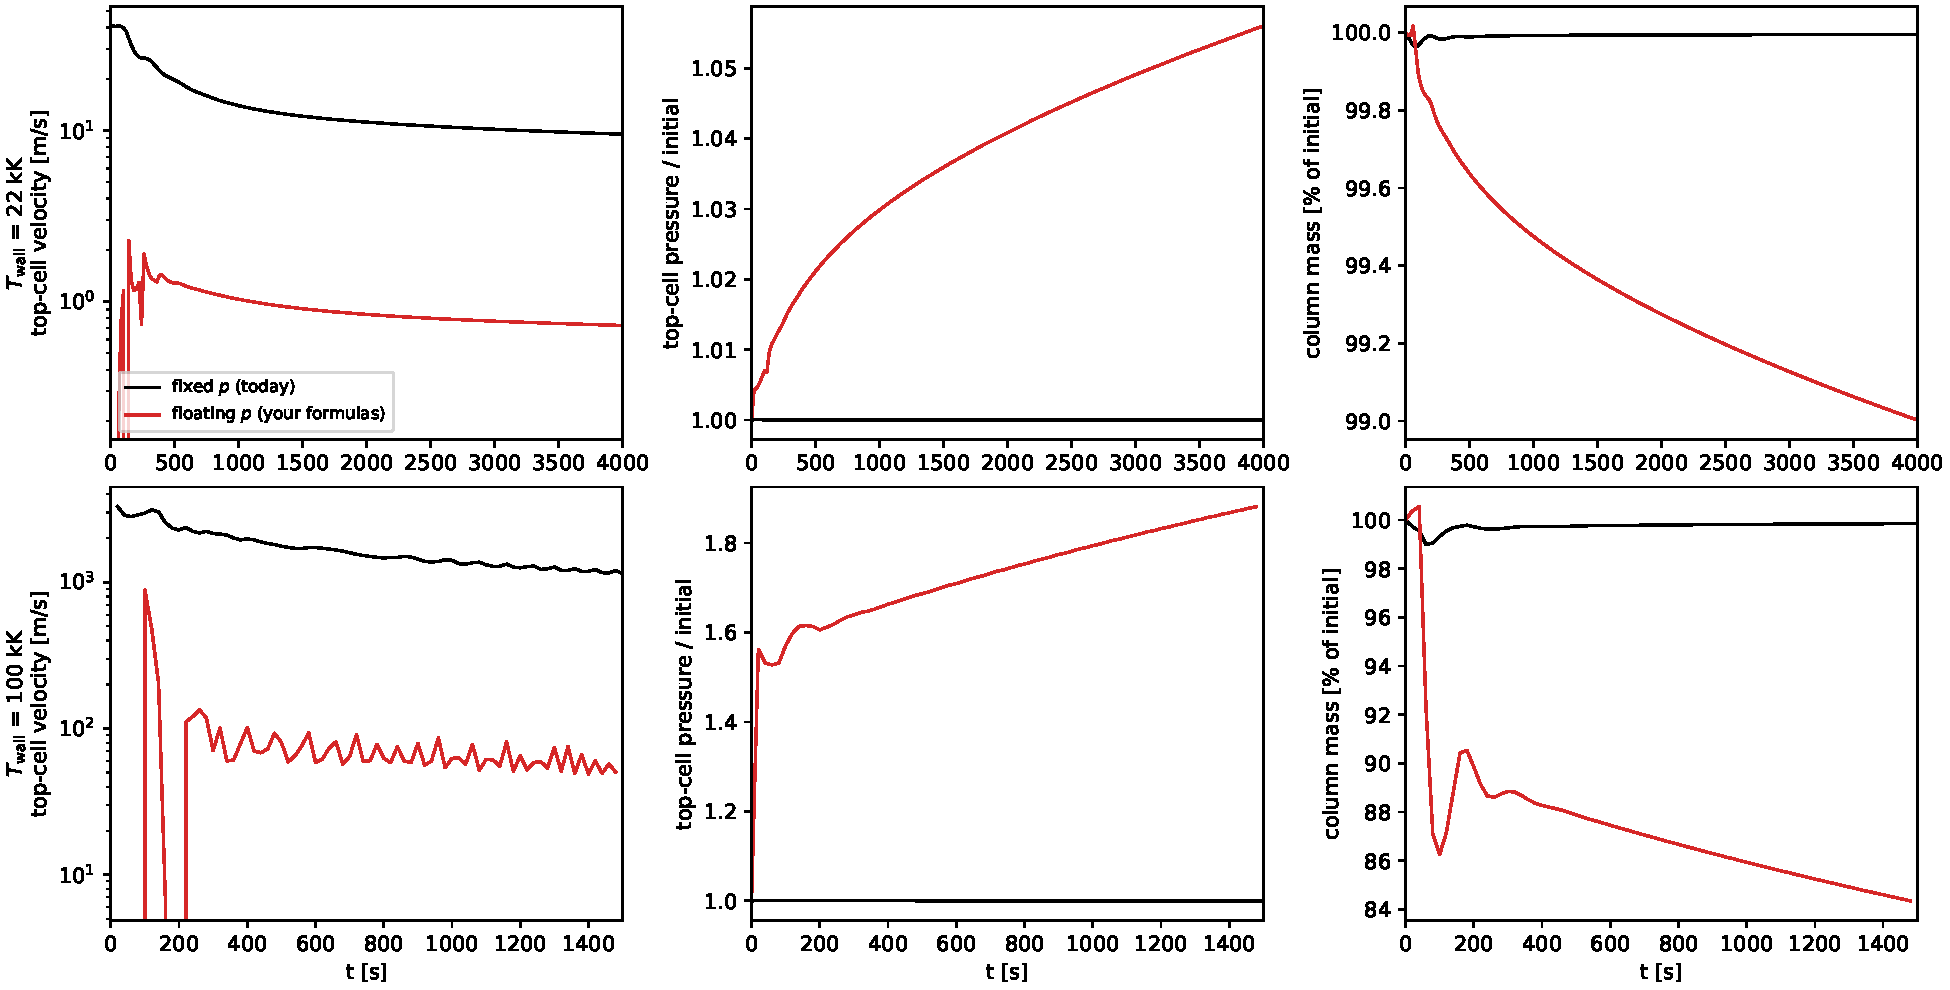
\includegraphics[width=0.88\textwidth]{outer_bc_rerun_timeseries.pdf}\\
  {\small Columns: top velocity, top pressure, column mass.}
\end{frame}

%----------------------------------------------------------------------
\begin{frame}{Result in numbers}
  \centering
  \begin{tabular}{@{}l r r@{}}
    \toprule
    & fixed $p$ & \textbf{floating $p$} \\
    \midrule
    \multicolumn{3}{@{}l}{\textit{22\,kK}} \\
    top mass flux [$10^{-10}$\,kg\,m$^{-2}$\,s$^{-1}$] & 2.74 & \textbf{0.22} \\
    bottom mass flux & 2.75 & \textbf{$-$2.30} \\
    top pressure / initial & 1.00 & \textbf{1.06} \\
    \midrule
    \multicolumn{3}{@{}l}{\textit{100\,kK}} \\
    top mass flux [$10^{-9}$\,kg\,m$^{-2}$\,s$^{-1}$] & 7.92 & \textbf{0.69} \\
    bottom mass flux & 8.05 & \textbf{$-$6.24} \\
    top pressure / initial & 1.00 & \textbf{1.88} \\
    column mass & 99.8\,\% & \textbf{84\,\%} \\
    \bottomrule
  \end{tabular}
  \vspace{0.6em}

  {\small Averages over the last 500\,s; positive = upward.}
\end{frame}

%----------------------------------------------------------------------
\begin{frame}{At 100\,kK the transition region sinks}
  \centering
  Height of the 7\,kK isotherm [km]:
  \vspace{0.6em}

  \begin{tabular}{@{}l r r r r@{}}
    \toprule
    $t$ [s] & 0 & 200 & 800 & 1480 \\
    \midrule
    fixed $p$    & 2136 & 2136 & 2127 & 2120 \\
    floating $p$ & 2136 & \textbf{2003} & 1978 & \textbf{1956} \\
    \bottomrule
  \end{tabular}
  \vspace{0.8em}

  180\,km into the chromosphere. Movie: \texttt{outer\_bc\_rerun\_100kK.mp4}
\end{frame}

%----------------------------------------------------------------------
\begin{frame}{Why}
  \begin{itemize}
    \item \textbf{Top pressure rises}: heating raises the scale height; only the bottom
          anchors the level.
    \item \textbf{Mass exits at the bottom}: the only face that holds its pressure.
    \item \textbf{Evaporation collapses}: nothing holds the coronal pressure to push against.
  \end{itemize}
\end{frame}

%----------------------------------------------------------------------
\begin{frame}{Coupling to AWSoM-R: options}
  AWSoM-R's TR pressure comes from its static TR model, so taking it is partly circular.
  But the corona's demand for mass reaches us as pressure ($w_-$).
  \vspace{0.5em}
  \begin{enumerate}
    \item Keep: AWSoM-R gives $(T,p)$, we return $J$.
    \item Exchange waves: AWSoM-R gives $w_-$, we give $w_+$, $w_s$. (Untested)
    \item Give heat flux $q$ instead of $p$: $J = q/(h_{\rm top}-h_c)$ in steady state.
          Needs a slow relaxation of $p_b$. (Untested)
  \end{enumerate}
\end{frame}

%======================================================================
\begin{frame}
  \centering\Large Part 2: pulses at hot walls
\end{frame}

%----------------------------------------------------------------------
\begin{frame}{Pulses at 100\,kK: halve every cell}
  \centering
  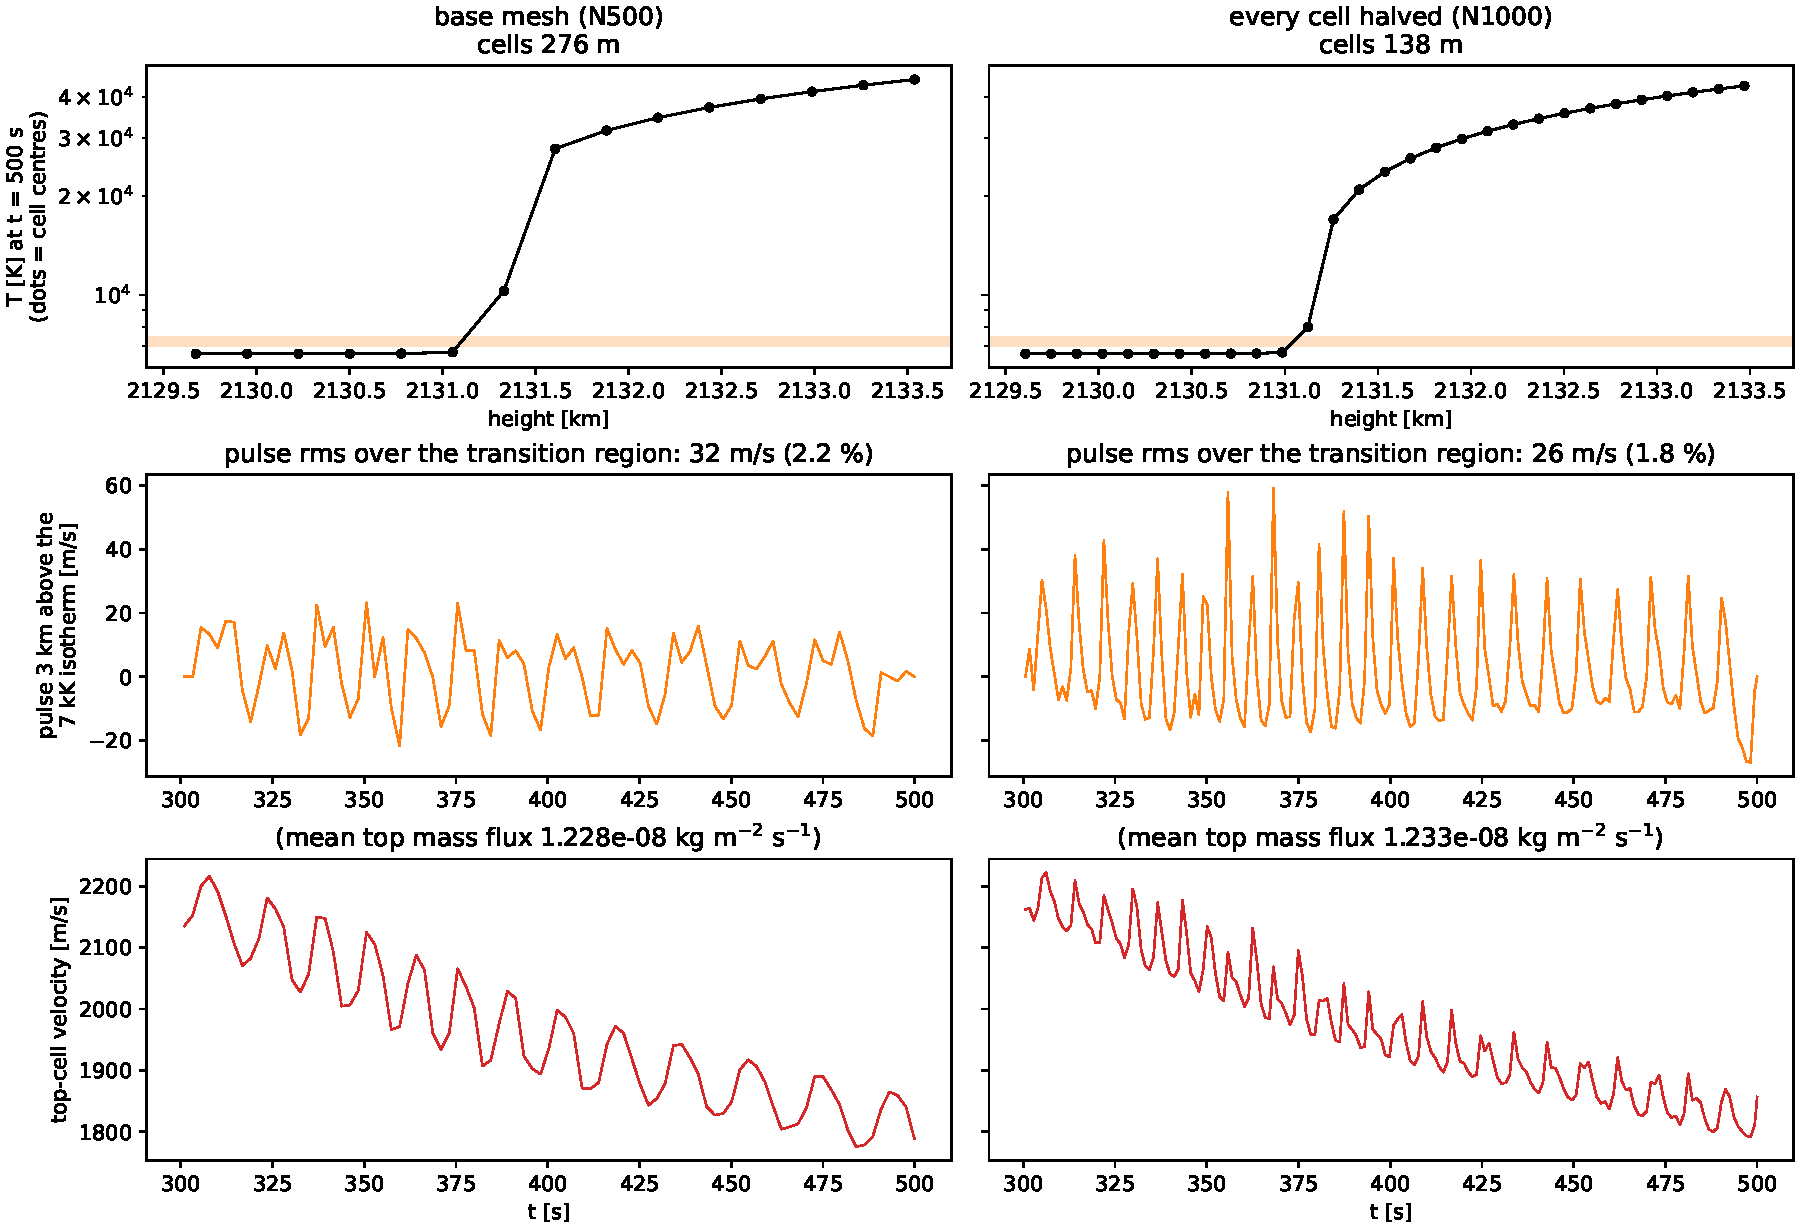
\includegraphics[width=0.62\textwidth]{tr_pulses_resolution.pdf}\\
  {\small Left: 276\,m cells. Right: 138\,m cells. Rows: temperature (dots = cells),
  velocity pulse in the transition region, top velocity.}\\[0.3em]
  Movie: \href{run:movies/tr_pulses_N500_vs_N1000_100kK.mp4}{\texttt{tr\_pulses\_N500\_vs\_N1000\_100kK.mp4}}
\end{frame}

%----------------------------------------------------------------------
\begin{frame}{What the comparison shows}
  \begin{itemize}
    \item Halving the cells \textbf{doubles the pulse frequency}: the pulses follow the
          grid $\Rightarrow$ numerical.
    \item Each pulse starts when the base of the transition region (7\,kK) enters a new cell.
    \item Amplitude only 20\,\% lower; mean mass flux unchanged (0.4\,\%).
  \end{itemize}
  \vspace{0.8em}
  \textbf{Next}: finer cells at the transition-region base, a different face formula for
  the heat flux, or TRAC.
\end{frame}

%----------------------------------------------------------------------
\begin{frame}{Why only at hot walls}
  Width of the ionization layer (7.0--7.5\,kK) in steady state:
  \[
    \Delta s \;\approx\; \frac{\int_{7.0\,\rm kK}^{7.5\,\rm kK}\kappa\,dT}{J\,(h-h_c)}
    \;\propto\; \frac{1}{J}
  \]
  Hotter wall $\to$ faster evaporation $J$ $\to$ thinner layer.
  \vspace{0.5em}
  \begin{center}
  \begin{tabular}{@{}r r l l@{}}
    \toprule
    $T_{\rm wall}$ & $J$ [kg\,m$^{-2}$\,s$^{-1}$] & layer vs 276\,m cell & pulses \\
    \midrule
    22\,kK  & $5.7\times10^{-10}$ & $\approx$2.6\,km, several cells & none \\
    45\,kK  & $2.4\times10^{-9}$  & thinner than one cell & yes \\
    100\,kK & $1.1\times10^{-8}$  & $\approx$30\,m, $\sim$1/10 cell & yes, largest \\
    \bottomrule
  \end{tabular}
  \end{center}
  \vspace{0.3em}
  Once the layer is thinner than a cell, each cell flips from cold to hot at once:
  a pulse. To resolve it at 100\,kK: $\sim$25\,m cells ($10\times$ finer).
\end{frame}

%----------------------------------------------------------------------
\begin{frame}{Movies (\texttt{movies/})}
  \begin{itemize}
    \item \href{run:movies/outer_bc_rerun_22kK.mp4}{\texttt{outer\_bc\_rerun\_22kK.mp4}}: fixed vs floating $p$, 22\,kK
    \item \href{run:movies/outer_bc_rerun_22kK_pressure.mp4}{\texttt{outer\_bc\_rerun\_22kK\_pressure.mp4}}: same, pressure above 2100\,km only
    \item \href{run:movies/outer_bc_rerun_100kK.mp4}{\texttt{outer\_bc\_rerun\_100kK.mp4}}: same, 100\,kK (TR sinks)
    \item \href{run:movies/tr_pulses_N500_vs_N1000_100kK.mp4}{\texttt{tr\_pulses\_N500\_vs\_N1000\_100kK.mp4}}: two resolutions
  \end{itemize}
\end{frame}

%======================================================================
\begin{frame}{Summary and questions}
  \begin{enumerate}
    \item \textbf{Boundary}: with conduction the top needs 2 conditions. Fixing only $T$
          loses evaporation ($12\times$) and drains the column.
    \item \textbf{Pulses}: numerical; they follow the grid. Mean flux unaffected.
  \end{enumerate}
  \vspace{0.8em}
  \textbf{Questions}
  \begin{itemize}
    \item Is the count with conduction right (slide~\ref{fr:count2})?
    \item What should AWSoM-R give us: $p$, $w_-$, or $q$?
    \item For the pulses: finer mesh near the transition region, or TRAC?
  \end{itemize}
\end{frame}

\end{document}
